	\documentclass[twoside]{article}
\usepackage{../../estilo-ejercicios}
\setcounter{section}{0}
\newtheorem{defin}{Definition}[section]
\newtheorem{lem}[defin]{Lemma}
\newtheorem{propo}[defin]{Proposition}
\newtheorem{thm}[defin]{Theorem}
\newtheorem{eje}[defin]{Example}
\newtheorem{obs}[defin]{Observación}
\renewcommand{\baselinestretch}{1,3}
%--------------------------------------------------------
\begin{document}

\title{Characterization of Extremal Antipodal Polygons}
\author{Javier Aguilar Martín}
\maketitle

%\varprojlim
%\varinjlim
\section{Introduction}

For a point $p=(x_1,x_2)\in\R^2$, let $p'=(-x_1,-x_2)$ be the antipodal point of $p$.

\begin{defin}
A set of $2n$ ($n\geq 3$) points on the unit circle centered at the origin is called an \emph{antipodal point set} if for every point $p\in S$, also $p'\in S$. Let $S=\{p_1,p_1'\dots,p_n,p_n'\}$ such set. An \emph{antipodal polygon} on $S$ is a convex polygon  having as vertices one point from each pair $(p_i,p_i')$. A \emph{thin} antipodal polygon $P$ is an antipodal polygon whose verticies are consecutive points on the circle. For $n$ odd, a \emph{thick} antipodal polygon $P$ is an antipodal polygon such that there is a point of $S$ between every two vertices of $P$. For $n$ even there is exactly one pair of vertices of $P$ which are consecutive on the circle. 
\end{defin}

\begin{figure}[h!]
\centering
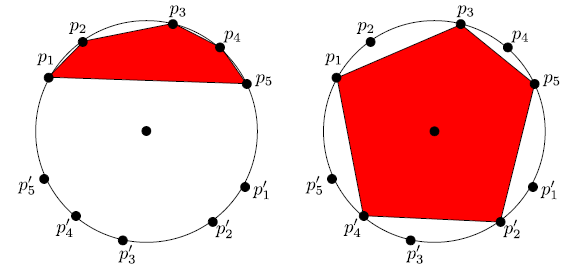
\includegraphics[scale=0.7]{fig1}
\caption{A thin (left) and a thick (right) antipodal polygon.}
\end{figure}
 
 
 Note that an antipodal polygon $P$ can be neither thick or thin, but it cannot be both at the same time. Moreover, a thin antipodal polygon does not contain the origin and a non-thin polygon always contains it (not choosing one point of $S$ implies choosing its antipodal). 
 
We will consider the following questions:
\begin{itemize}
\item Does a thick antipodal polygon always have larger area than a thin antipodal polygon?
\item How efficiently can one compute an antipodal polygon with minimal (maximal)
area?
\item What can be said about antipodal polygons in higher dimensions?
%•
\end{itemize}

\subsection{Related Work}
NO HAY TIEMPO PA ESTO

\subsection{Results}\label{claim}
We will prove the following general result:\\

\emph{Claim} Given an antipodal point set $S ⊂ \R^2$, every thin antipodal polygon on $S$ has
less area than any non-thin antipodal polygon on $S$.\\

In addition we show that the 2-dimensional case is special in the sense that the
above result can not be generalized to higher dimensions.

The analogue result holds for thick antipodal polygons when $n$ is odd but for $n$ even we provide an example of
an antipodal non-thick polygon having larger area than a thick antipodal polygon. However, we are able to prove the following result:\\

\emph{Claim} Given an antipodal point set $S ⊂ \R^2$, for every non-thick antipodal polygon
on $S$ there exists a thick antipodal polygon on $S$ with larger area.\\

Note that above claims imply that an antipodal polygon with minimum (resp. maximum)
area is thin (resp. thick). As a consequence, we will show that the extremal
problems for antipodal polygons can be solved in linear time.

\section{Thin Antipodal Polygons}
Assume that the clockwise circular order of $S$ around the origin is $p_1, p_2, \dots , p_n,
p'_1, p'_2,\dots , p'_n$. For every point $q$ in $S$, let $P_q$ be the thin antipodal polygon that
contains as vertices $q$ and the next $n −1$ clockwise consecutive points of $S$. Note that
all thin antipodal polygons are of this form and that $P_q$ and $P_{q'}$ differ only by a rotation around the origin. 

The next lemma characterizes triangles that contain a given point of S and maximize
the area.

\begin{lem}\label{1}
For a point $p ∈ S$ let $l$ be the line containing $p$ and $p'$. Let $τ$ be the triangle
determined by $p$, and its two neighbors in $S$. Among all triangles that have as vertices
$p$ and one point of $S$ in each of the two half-planes defined by $l$, $τ$ has strictly the
smallest area.
\end{lem}
\begin{proof}
Let $τ'$ be a triangle with vertices in $S$, containing $p$ as a vertex and with a vertex
in each of the two half-planes defined by $l$. Assume that $τ'$ is different from $τ$. Let
$b$ be the side opposite to $p$ in $τ$ and $b'$ be the side opposite to $p$ in $τ'$. Note that $b'$
is at least as large as $b$, because $S$ is an antipodal point set and $l$ contains the origin.
The height of $τ'$ with respect to $p$ is larger than the height of $τ$ with respect to $p$, as
otherwise $b'$ would have to intersect $b$, which is not possible by construction. Thus
the area of $τ'$ is larger than the area of $τ$.

HACER UN DIBUJITO
\end{proof}


We split the proof of the first claim of \ref{claim} into the three cases $n = 3$, $n = 4$, and $n ≥ 5$.

\begin{lem}\label{2}
For $n = 3$, every thin antipodal polygon on $S$ has area strictly less than
that of any non-thin antipodal polygon on $S$.
\end{lem}
\begin{proof}
In this case the only non-thin polygons are the two triangles $τ$ and $τ'$ with vertex
sets $\{p_1, p_2', p_3\}$ and $\{p_1', p_2, p_3'\}$, respectively. Note that $τ$ has the same area as $τ'$.
In addition, by Lemma \ref{1}, $τ$ has larger area than $P_{p_2}$ and $τ'$ has larger area than $P_{p_1}$
and $P_{p_3}$.

HACER UN DIBUJITO
\end{proof}


\begin{lem}\label{3}
For $n = 4$, every thin antipodal polygon on $S$ has area strictly less than
that of any non-thin antipodal polygon on $S$.
\end{lem}


\begin{thm}
Every thin antipodal polygon on $S$ has less area than any non-thin antipodal
polygon on $S$.
\end{thm}

The idea of the proof is induction on $n$ with lemmas \ref{2} and \ref{3} as base case. For $n\geq 5$, consider a triangulation $T$ of $S$, and by analysing the thin triangles of $T$ one can reduce the problem to the case $n-1$. 


\section{Thick Antipodal Polygons}
ULISES

\section{Higher Dimensions: Antipodal Polytopes}
ULISES


 \section{Open Problems}
 NO LO ENTIENDO, PREGUNTARLE AL PROFESOR
\end{document}
